
\section{Roda Omnidirecional}

A roda omnidirecional aparece em vários modelos na literatura, tais como no design de J. Graboweicki em 1919
\cite{patent_US1305535A} e o de Josef Blumrich em 1972 \cite{patent_US3789947A}. A roda consiste de rolos
perpendiculares à  sua direção de giro, cuja presença tem como efeito conferir à roda a capacidade de se locomover em
qualquer direção no seu plano. Essa capacidade é o que confere aos robôs aqui discutidos suas características
holonômicas, uma vez que as restrições de movimento a que eles estão sujeitos está normalmente atrelada à construção das
rodas \cite{TAKAHASHI}.

\begin{figure}[h] 
	\centering
	\caption{Modelo de uma Roda Omnidirecional}
	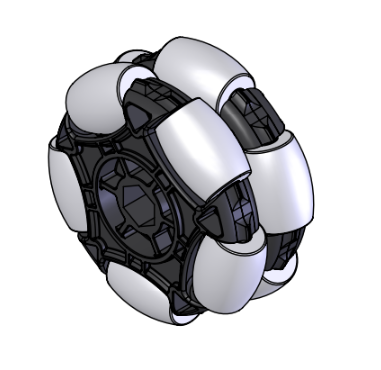
\includegraphics[width=0.5\textwidth]{figures/omniwheel}
	\fonte{\cite{draw_omniwheel}}
\end{figure}

A relação entre velocidade linear e angular da roda é dada por:

\[V_{w1} = \omega_{w1}\cdot r \] 

em que $V_{w}$ é velocidade linear da roda, $r$ o raio da roda, $\omega_{w} $ e é a velocidade angular da roda.

Uma variação da roda omnidirecional é a roda mecanum, criada por Bengt Ilon \cite{patent_US3876255A} - a diferença
fundamental entre elas é a construção dos rolos ligados à estrutura central - os quais, no caso da roda mecanum, são
posicionados a 45°.

\subsection{Obtencão da roda omnidirecional}

Inicialmente, utilizaram-se rodas omnidirecionais fabricadas fora do Brasil e disponíveis para importação. Também é
possível adquirir o mesmo modelo com revendedores nacionais.
Tal modelo possui diâmetro de 58mm, largura de 26mm e possui um acoplamento para eixo de 4mm de diâmetro. Essas
dimensões eram adequadas nos primeiros testes de construção do robô, enquanto se estava usando motores DC. Uma vez que
se passou a empregar motores de passo Nema 17 (mudança discutida na seção \ref{secao_motores}), contudo, as rodas não eram
mais compatíveis com o eixo e as dimensões dos motores.

\begin{figure}[h]
	\centering
	\caption{Roda omnidirecional usada inicialmente}
	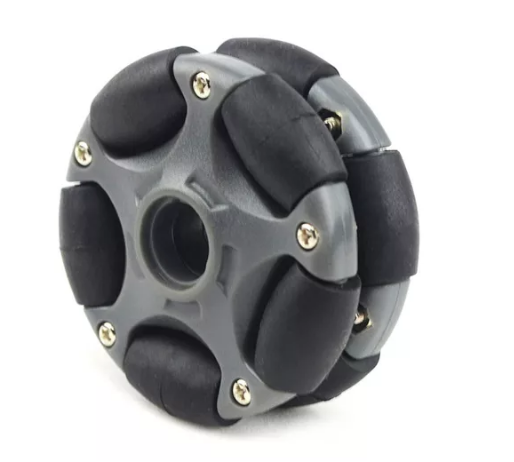
\includegraphics[width=0.5\textwidth]{figures/roda_china.png}	
	\fonte{\cite{omin_wheel_produto_2}}
\end{figure}

A mudança de requisitos para as rodas levou à criação de um design próprio, conforme as
\autorefmany{new_wheel_cad_design, estudo_design, design_solid, design_impressao, wheel_assembling}.
As novas rodas possuem 69mm de diâmetro e 27mm de largura,
e foram fabricadas com impressora
3D (com filamento PLA), parafusos sextavado de M3, e reutilizando os rolamentos das rodas de 58mm.

\begin{figure}[h]
	\centering
	\caption{Processo de design da nova roda - AutoCAD}
	\label{new_wheel_cad_design}
	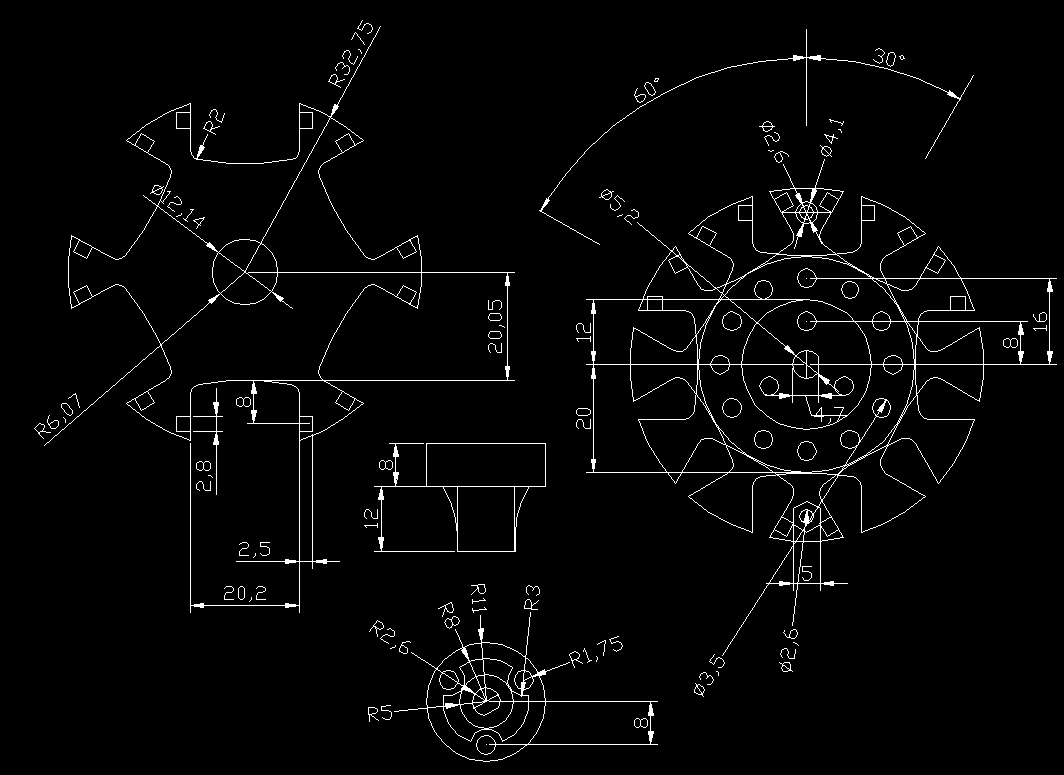
\includegraphics[width=0.9\textwidth]{figures/roda_processo_desing_passo1}
	\fonte{Própria}
\end{figure}

\begin{figure}[h]
	\centering
	\caption{Estudo e testes do design da nova roda}
	\label{estudo_design}
	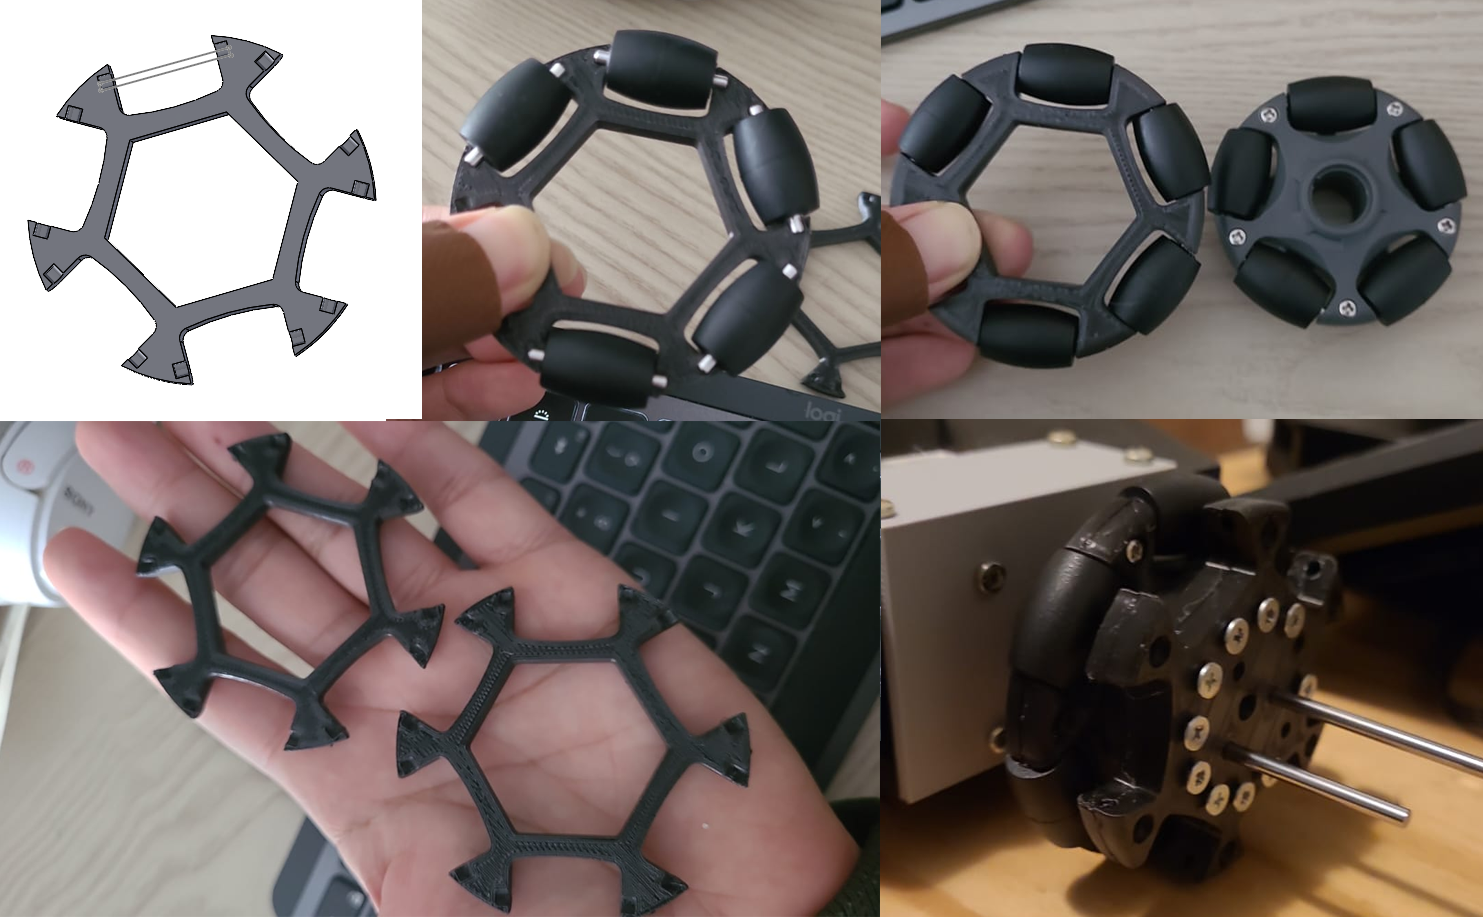
\includegraphics[width=0.9\textwidth]{figures/estudo_roda}
	\fonte{Própria}
\end{figure}

\begin{figure}[h]
	\centering
	\caption{Design final - Solidworks}
	\label{design_solid}
	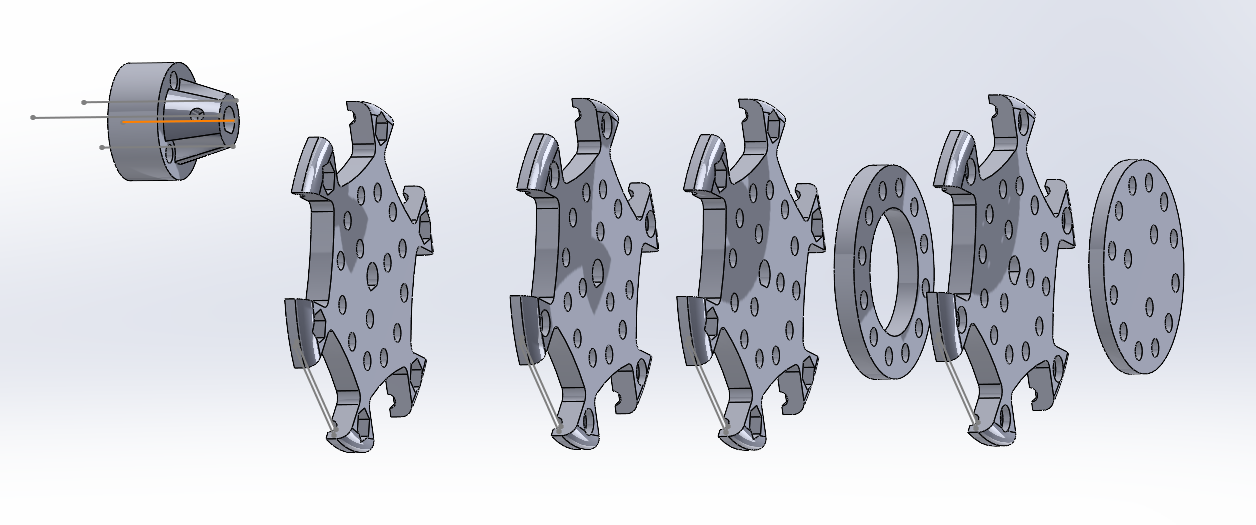
\includegraphics[width=0.9\textwidth]{figures/roda_processo_desing_passo2}
	\fonte{Própria}
\end{figure}

\begin{figure}[h]
	\centering
	\caption{Design final - Preparação para impressão}
	\label{design_impressao}
	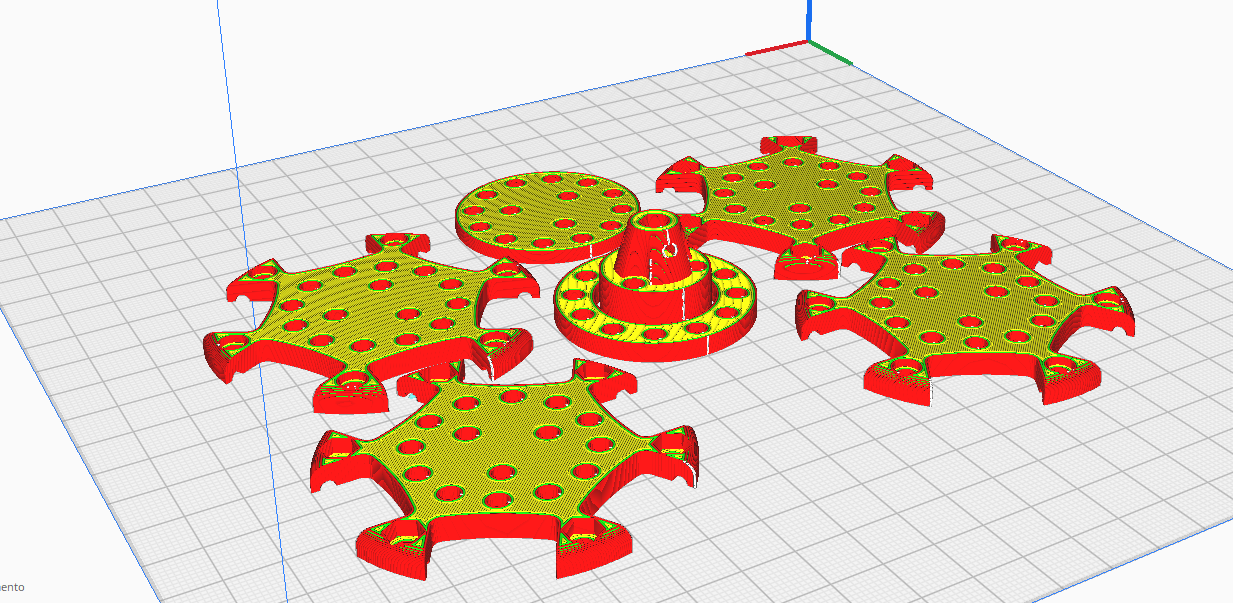
\includegraphics[width=0.9\textwidth]{figures/roda_processo_desing_passo3}
	\fonte{Própria}
\end{figure}

\begin{figure}[h]
	\centering
	\caption{Montagem da roda}
	\label{wheel_assembling}
	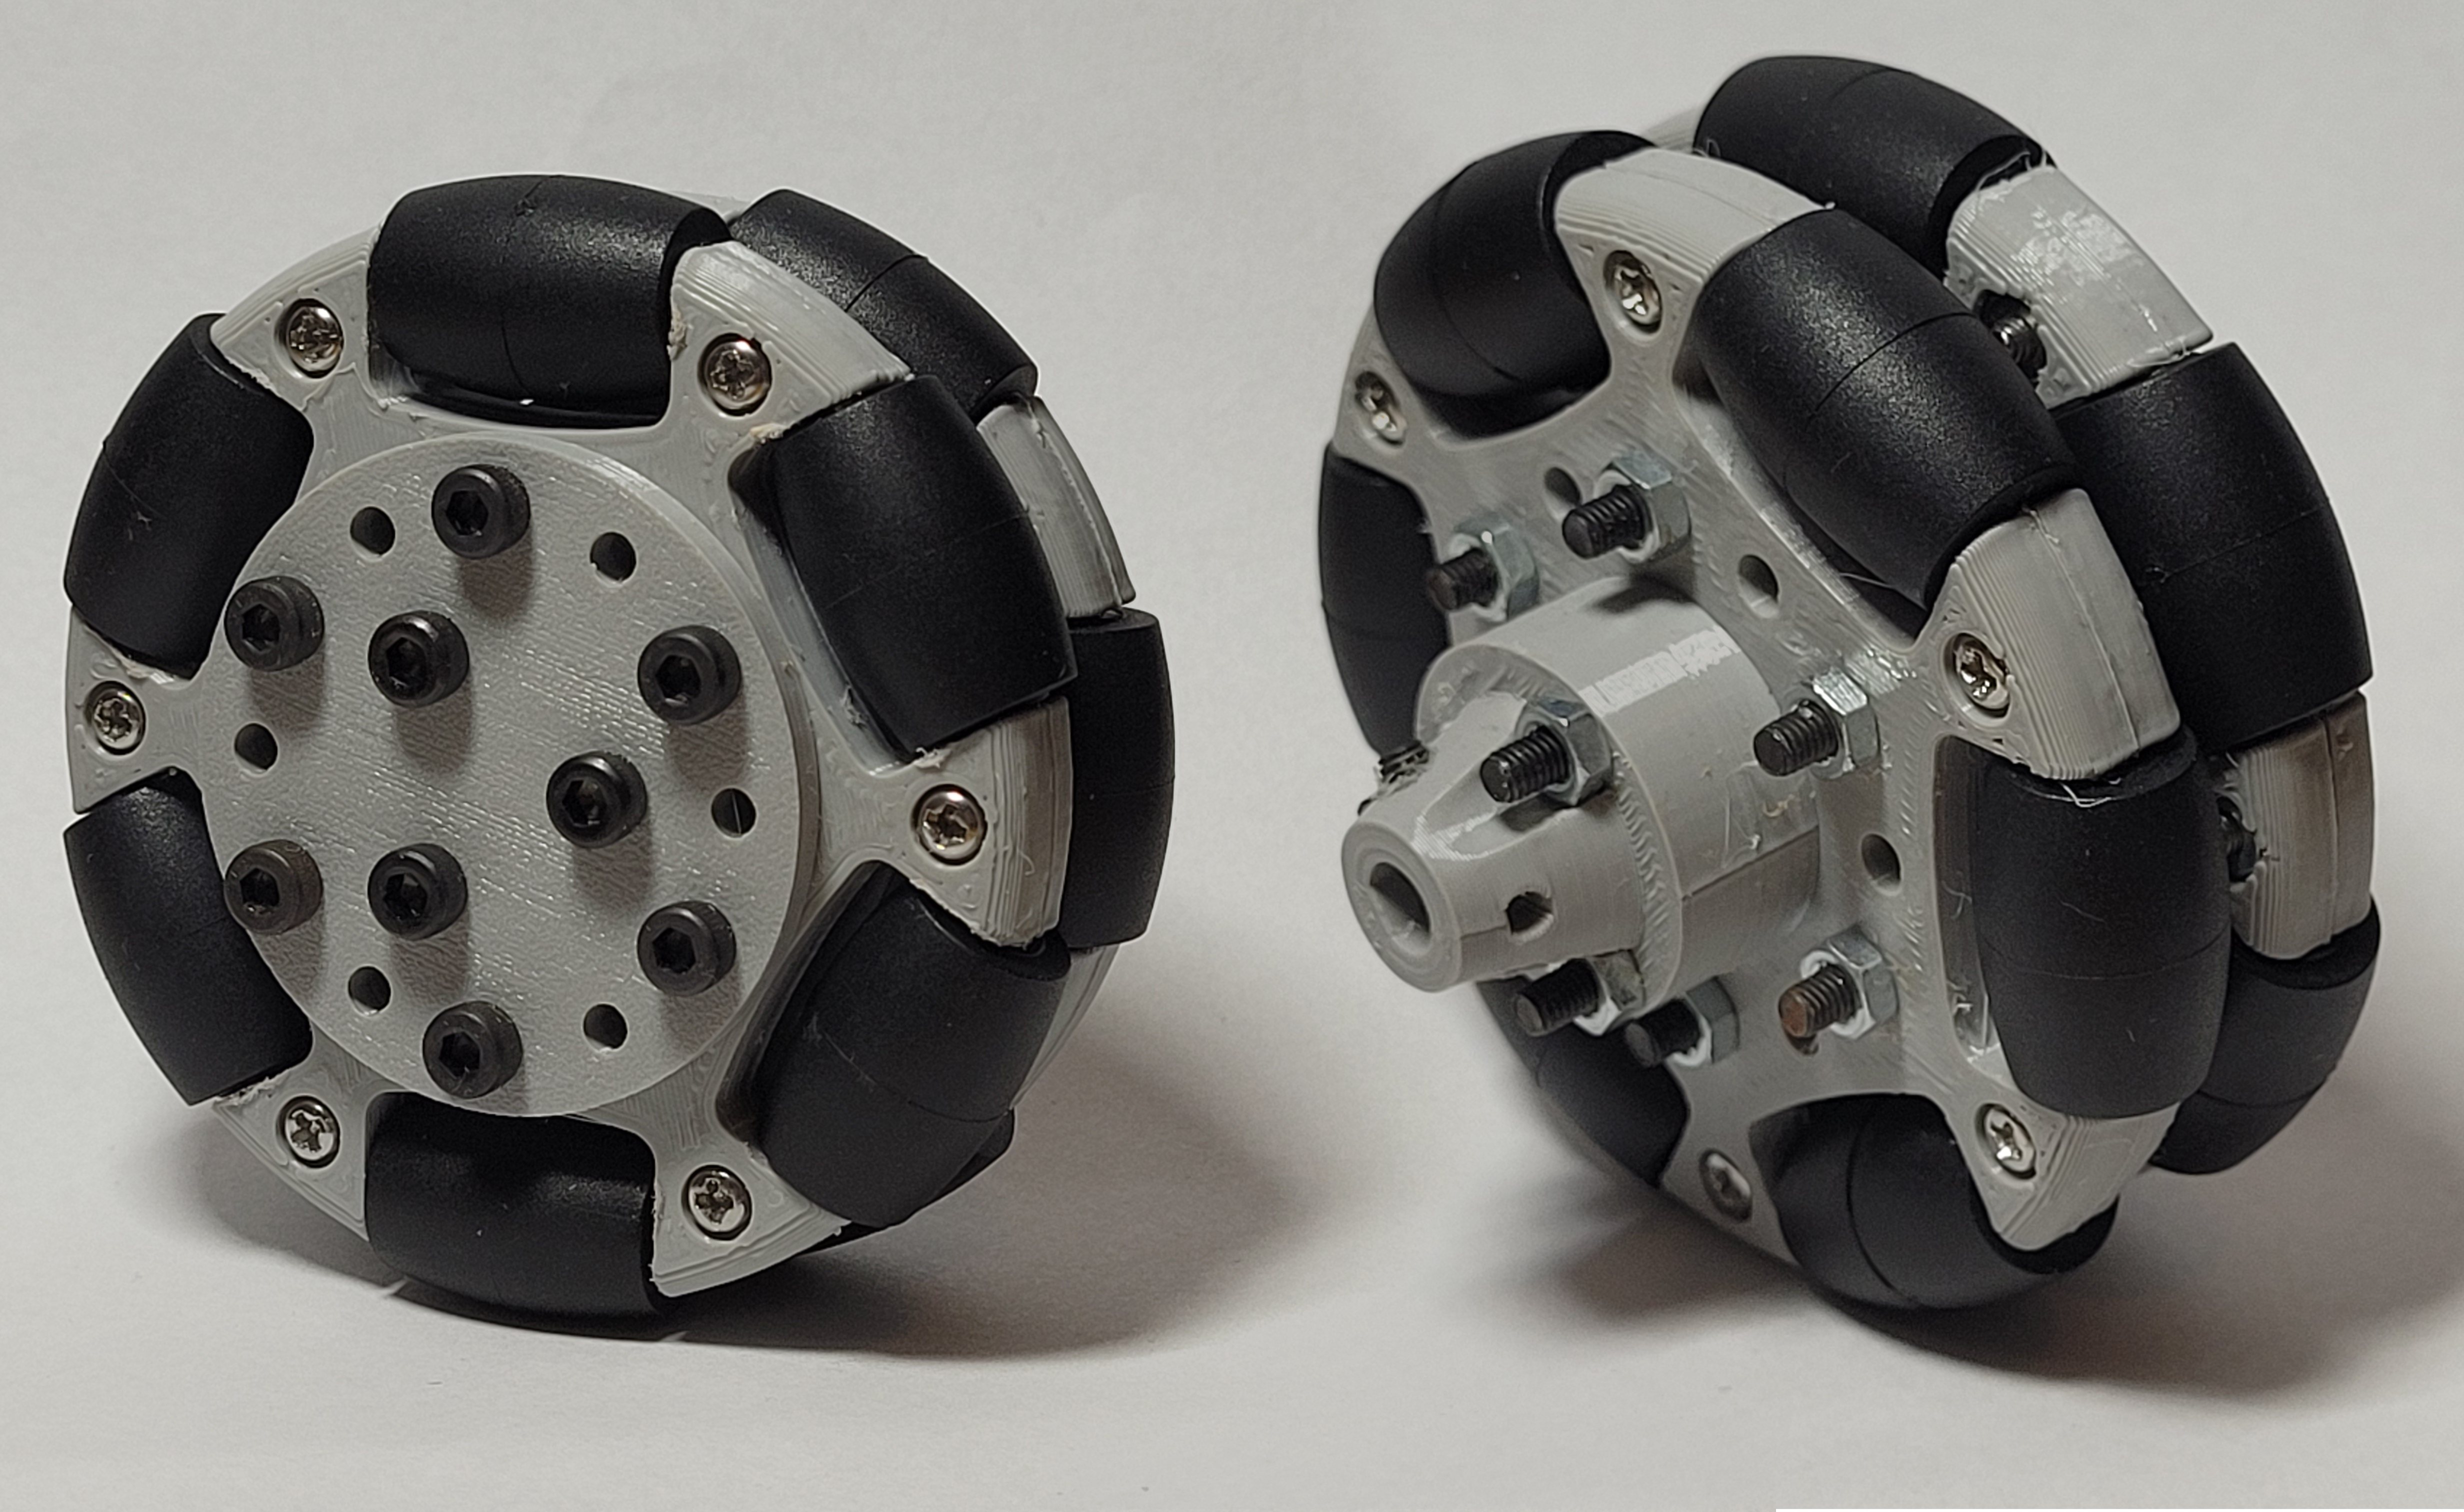
\includegraphics[width=0.9\textwidth]{figures/roda_processo_desing_passo4}
	\fonte{Própria}
\end{figure}